
\section{\BookRecordIndex{T0257}粘合映射的构造}\label{sec:10-5}

本节定义\BookRecordIndex{T0257}粘合映射 $\iota_c^R$，并证明它具有定理~\ref{thm:10-1-2} 的性质
(i)、(ii) 与 (iii)。如导言所述，其思路是在\BookRecordIndex{T0394}预粘合
$u^R:=u^{\delta,R}$ 附近应用\BookRecordIndex{T0380}隐函数定理，找到一条真正的全纯曲线
\[
  \widetilde u^R:=\iota_c^R(u^0,u^\infty).
\]
为此必须证明：只要 $\delta>0$ 充分小而 $\delta R$ 充分大，
\BookRecordIndex{T0128}弗雷德霍姆算子 $D_{u^R}$ 就满射，并且具有一致有界的\BookRecordIndex{T0392}右逆。

\paragraph{\BookRecordIndex{T0392}右逆的估计。}
第一步是沿用 Donaldson--Kronheimer \srcite{88} 的方法构造\BookRecordIndex{T0196}近似右逆
$T_{u^R}$。下面的命题概括它的主要性质。回忆式~\eqref{eq:10-1-5}：
$\mathcal A(\delta_0)$ 表示实数偶对 $(\delta,R)$ 的集合，其中
$0<\delta<\delta_0$ 且 $\delta R>1/\delta_0$。

\begin{proposition}\label{prop:10-5-1}
设 $A^0,A^\infty\in H_2(M;\mathbb Z)$，并设
\[
  (J^0,J^\infty)\in
  \mathcal J_{\mathrm{reg}}(S^2;A^{0,\infty}).
\]
固定常数 $c>0$ 与 $p>2$。则存在常数 $\delta_0>0$、$c_0>0$，以及一个
光滑映射；它为每个 $u=(u^0,u^\infty)\in\mathcal M(c)$ 和每个
$(\delta,R)\in\mathcal A(\delta_0)$ 指派有界线性算子
\[
  T_{u^R}:
  L^p\bigl(S^2,\Lambda^{0,1}\otimes_{J^R}(u^R)^*TM\bigr)
  \longrightarrow
  W^{1,p}\bigl(S^2,(u^R)^*TM\bigr),
\]
这里 $u^R:S^2\to M$ 是由式~\eqref{eq:10-2-1} 和~\eqref{eq:10-2-2}
定义的\BookRecordIndex{T0395}预粘合曲线，并且对每个
$\eta\in L^p(S^2,\Lambda^{0,1}\otimes_{J^R}(u^R)^*TM)$ 都有
\begin{equation}\label{eq:10-5-1}
  \bigl\|D_{u^R}T_{u^R}\eta-\eta\bigr\|_{0,p,R}
  \le\frac12\|\eta\|_{0,p,R},
  \qquad
  \bigl\|T_{u^R}\eta\bigr\|_{1,p,R}
  \le\frac{c_0}{2}\|\eta\|_{0,p,R}.
\end{equation}
\end{proposition}

在开始证明之前，先引入一些简化记号。我们先改述 $J$ 的\BookRecordIndex{T0408}正则性条件。对
$u:S^2\to M$ 和 $J=\{J_z\}_{z\in S^2}$，简记
\[
  W_u^{1,p}:=W^{1,p}(S^2,u^*TM),
  \qquad
  L_{u,J}^p:=L^p(S^2,\Lambda^{0,1}\otimes_Ju^*TM).
\]
给定满足 $u^0(0)=u^\infty(\infty)$ 的映射
$u^0,u^\infty:S^2\to M$，记
\[
  W_{u^{0,\infty}}^{1,p}
  :=\bigl\{(\xi^0,\xi^\infty)\in
  W_{u^0}^{1,p}\times W_{u^\infty}^{1,p}
  \bigm|\xi^0(0)=\xi^\infty(\infty)\bigr\}.
\]
最后这个定义只有在 $p>2$ 时才有意义，因为只有此时 $W^{1,p}$ 截面才连续，
从而可以在一点处求值。定义~\ref{def:10-1-1} 中的\BookRecordIndex{T0166}横截性假设蕴含算子
\[
  D_{0,\infty}:=D_{u^0,u^\infty}:
  W_{u^{0,\infty}}^{1,p}
  \longrightarrow L_{u^0,J^0}^p\times L_{u^\infty,J^\infty}^p
\]
为满射；这里
\[
  D_{0,\infty}(\xi^0,\xi^\infty)
  :=(D_{u^0}\xi^0,D_{u^\infty}\xi^\infty).
\]
为说明这一点，对 $a=0,\infty$ 给定 $\eta^a\in L_{u^a,J^a}^p$，
并选取 $\xi^a\in W_{u^a}^{1,p}$ 使 $D_{u^a}\xi^a=\eta^a$。再选取切向量
$\zeta^a\in T_{u^a}\mathcal M(A^a;J^a)$，使
\[
  d\operatorname{ev}(u^0,u^\infty)(\zeta^0,\zeta^\infty)
  =(\zeta^0(0),\zeta^\infty(\infty))
  \in(\xi^0(0),\xi^\infty(\infty))+T_{(x,x)}\Delta.
\]
于是 $(\xi^0-\zeta^0,\xi^\infty-\zeta^\infty)$ 属于
$W_{u^{0,\infty}}^{1,p}$，并且在 $D_{0,\infty}$ 下的像仍为
$(\eta^0,\eta^\infty)$。所以 $D_{0,\infty}$ 有一个随偶对
$(u^0,u^\infty)$ 光滑变化的\BookRecordIndex{T0392}右逆；当该偶对在紧空间
\[
  \mathcal M(c):=
  \mathcal M(A^{0,\infty};J^{0,\infty},c)
\]
中变化时，这个\BookRecordIndex{T0392}右逆满足一致界。\sourcefootnote{原书在这里把\BookRecordIndex{T0226}连通对空间缩写为
$\mathcal M(A^{0,\infty};J,c)$；但固定数据始终是偶对
$J^{0,\infty}=(J^0,J^\infty)$，且本节下一节也明确采用
$\mathcal M(A^{0,\infty};J^{0,\infty},c)$，故补出上标。}

更准确地说，令
\[
  \mathcal W_{u^{0,\infty}}\subset W_{u^{0,\infty}}^{1,p}
\]
为 $\ker D_{0,\infty}$ 的 $L^2$-正交补。于是
$D_{0,\infty}$ 在 $\mathcal W_{u^{0,\infty}}$ 上的限制是双射有界线性算子，
所需算子就是其逆：
\[
  Q_{0,\infty}:=Q_{u^0,u^\infty}
  :=\left(D_{0,\infty}\big|_{\mathcal W_{u^{0,\infty}}}\right)^{-1}.
\]
它随偶对 $(u^0,u^\infty)$ 光滑变化；其范数的一致估计来自
$\mathcal M(c)$ 的\BookRecordIndex{T0192}紧性。注意，算子的定义域和值域实际上依赖
$(u^0,u^\infty)$。因此，为准确表述这种连续依赖性，必须对邻近的偶对
$(u^0,u^\infty)$、$(v^0,v^\infty)$，选取
$W_{u^{0,\infty}}^{1,p}$ 与 $W_{v^{0,\infty}}^{1,p}$ 之间的等同。
这可以像定理~\ref{thm:3-5-2} 的证明那样，沿短测地线作\BookRecordIndex{T0263}平行移动。

现在考虑注~\ref{rem:10-2-2} 中定义的映射
$u^{0,r},u^{\infty,r}$，仍令 $r:=\delta R$。它们是
$u^0,u^\infty$ 的 $W^{1,p}$-小扰动，因此可以把
$W_{u^{0,\infty}}^{1,p}$ 看作沿这些\BookRecordIndex{T0373}压平曲线的向量场空间
$W_{u^{0,\infty},r}^{1,p}$ 在 $r\to\infty$ 时的极限。此外，算子
\[
  D_{0,\infty,r}:=D_{u^{0,r},u^{\infty,r}}
\]
是\BookRecordIndex{T0346}线性化算子 $D_{0,\infty}:=D_{u^0,u^\infty}$ 的
$W^{1,p}$-小扰动，所以它也有\BookRecordIndex{T0392}右逆。以下选取唯一的\BookRecordIndex{T0392}右逆，使其像为
$\ker D_{0,\infty,r}$ 的 $L^2$-正交补，并记为
\[
  Q_{0,\infty,r}:=Q_{u^{0,r},u^{\infty,r}}:
  L_{u^{0,r},J^0}^p\times L_{u^{\infty,r},J^\infty}^p
  \longrightarrow W_{u^{0,\infty},r}^{1,p}.
\]
由于 $D_{0,\infty,r}$ 是 $D_{0,\infty}$ 的小扰动，它确实有一致有界的\BookRecordIndex{T0392}右逆。
不过，这里使用的是一族特定的\BookRecordIndex{T0392}右逆 $Q_{0,\infty,r}$，其像与
$\ker D_{0,\infty,r}$ 在 $L^2$ 意义下正交，所以还须为它们建立一致估计。
这些估计将在引理~\ref{lem:10-6-1} 中陈述和证明。这里所需的是如下结论：
对每个 $c>0$，都存在正数 $\delta_0,c_0$，使
\begin{equation}\label{eq:10-5-2}
  \|Q_{0,\infty,r}\eta\|_{W^{1,p}}
  \le c_0\|\eta\|_{L^p}
\end{equation}
对所有 $u=(u^0,u^\infty)\in\mathcal M(c)$、$r>1/\delta_0$ 及
\[
  \eta=(\eta^0,\eta^\infty)
  \in L_{u^{0,r},J^0}^p\times L_{u^{\infty,r},J^\infty}^p
\]
都成立。

现在的策略是用算子 $Q_{0,\infty,r}$，在 $r=\delta R$ 充分大时构造沿
\BookRecordIndex{T0395}预粘合曲线 $u^R$ 的算子 $D_{u^R}$ 的\BookRecordIndex{T0196}近似右逆 $T_{u^R}$，并为这些\BookRecordIndex{T0196}近似右逆
建立一致估计。

\begin{proof}[命题~\ref{prop:10-5-1} 的证明]
先定义算子
\[
  T_{u^R}:L_{u^R,J^R}^p\longrightarrow W_{u^R}^{1,p}.
\]
其构造可由下面的交换图概括，其中竖直映射由\BookRecordIndex{T0188}截断函数给出：
\begin{equation}\label{eq:10-5-3}
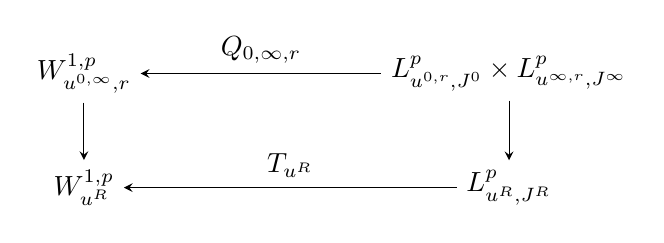
\begin{tikzpicture}[baseline=(current bounding box.center),>=stealth]
  \node (wt) at (0,1.45) {$W_{u^{0,\infty},r}^{1,p}$};
  \node (lt) at (5.4,1.45)
    {$L_{u^{0,r},J^0}^p\times L_{u^{\infty,r},J^\infty}^p$};
  \node (wb) at (0,0) {$W_{u^R}^{1,p}$};
  \node (lb) at (5.4,0) {$L_{u^R,J^R}^p$};
  \draw[<-] (wt) -- node[above] {$Q_{0,\infty,r}$} (lt);
  \draw[->] (wt) -- (wb);
  \draw[->] (lt) -- (lb);
  \draw[<-] (wb) -- node[above] {$T_{u^R}$} (lb);
\end{tikzpicture}
\end{equation}
下面给出细节。给定 $\eta\in L_{u^R,J^R}^p$，先沿圆周 $|z|=1/R$
截断 $\eta$，定义偶对
\[
  (\eta^0,\eta^\infty)
  \in L_{u^{0,r},J^0}^p\times L_{u^{\infty,r},J^\infty}^p
\]
如下：
\[
  \eta^0(z):=
  \begin{cases}
    \eta(z),&|z|\ge1/R,\\
    0,&|z|\le1/R,
  \end{cases}
  \qquad
  \eta^\infty(z):=
  \begin{cases}
    R^{-2}\eta(z/R^2),&|z|\le R,\\
    0,&|z|\ge R.
  \end{cases}
\]
$\eta^0,\eta^\infty$ 的不连续性不会造成问题，因为估计中只出现它们的
$L^p$-范数。第二步，定义
\[
  (\xi^0,\xi^\infty):=
  Q_{0,\infty,r}(\eta^0,\eta^\infty),
\]
并注意向量场 $\xi^0,\xi^\infty$ 有相同的中心值
\[
  \xi^0(0)=\xi^\infty(\infty)=:\xi_0\in T_{u^0(0)}M.
\]
第三步，令 $1-\beta_{\delta,R}:\mathbb C\to\mathbb R$ 为
引理~\ref{lem:10-4-1} 的\BookRecordIndex{T0188}截断函数，其中 $\delta,\varepsilon$ 分别换成
$\delta/R,1/R$。于是
\[
  \beta_{\delta,R}(z)=0\quad(|z|\le\delta/R),\qquad
  \beta_{\delta,R}(z)=1\quad(|z|\ge1/R),
\]
并且
\[
  \beta_{\delta,R}(z)
  :=\frac{\log(R|z|/\delta)}{\log(1/\delta)},
  \qquad \frac{\delta}{R}\le|z|\le\frac1R.
\]
第四步，定义 $T_{u^R}\eta:=\xi^R$，其中
\begin{equation}\label{eq:10-5-4}
\xi^R(z):=
\begin{cases}
\xi^0(z),
  & |z|\ge\dfrac1{\delta R},\\[3pt]
\xi^0(z)+\beta_{\delta,R}\!\left(\dfrac1{R^2z}\right)
  \bigl(\xi^\infty(R^2z)-\xi_0\bigr),
  & \dfrac1R\le|z|\le\dfrac1{\delta R},\\[6pt]
\xi^0(z)+\xi^\infty(R^2z)-\xi_0,
  & |z|=\dfrac1R,\\[3pt]
\xi^\infty(R^2z)+\beta_{\delta,R}(z)\bigl(\xi^0(z)-\xi_0\bigr),
  & \dfrac{\delta}{R}\le|z|\le\dfrac1R,\\[6pt]
\xi^\infty(R^2z),
  & |z|\le\dfrac{\delta}{R}.
\end{cases}
\end{equation}

理解这个定义最容易的情形是中心值 $\xi_0$ 为零，且 $z$ 位于\BookRecordIndex{T0170}环域
\[
  \frac{\delta}{R}\le|z|\le\frac1{\delta R}=\frac1r.
\]
在这个\BookRecordIndex{T0170}环域中，映射 $u^{0,r}(z)$、$u^{\infty,r}(R^2z)$ 与 $u^R(z)$
都取常值
\[
  x:=u^0(0)=u^\infty(\infty),
\]
而
\[
  \xi^R:\left\{\frac{\delta}{R}\le|z|\le\frac1{\delta R}\right\}
  \longrightarrow T_xM
\]
正是函数
$\beta_{\delta,R}(z)\xi^0(z)$ 与
$\beta_{\delta,R}(1/R^2z)\xi^\infty(R^2z)$ 的叠加。关键在于：第一项中的
\BookRecordIndex{T0188}截断函数 $\beta_{\delta,R}(z)$ 只在 $|z|\le1/R$ 的区域内起作用，而在这里
\[
  D_{0,r}\xi^0:=D_{u^{0,r}}\xi^0=0.
\]
见图~\ref{fig:10-5-1}。第二项同理，因为该构造关于
$u^{0,r}$ 与 $u^{\infty,r}$ 完全对称。当 $\xi_0\ne0$ 时，也可以按同样方式
理解公式，只须把“原点”换成 $\xi_0$。

\begin{figure}[htbp]
\centering
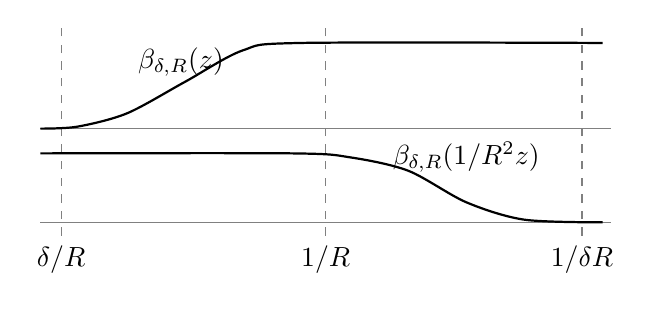
\begin{tikzpicture}[x=1.05cm,y=0.85cm]
  \draw[gray] (0.3,1.55)--(7.2,1.55);
  \draw[gray] (0.3,0.15)--(7.2,0.15);
  \draw[dashed,gray] (0.55,-0.05)--(0.55,3.05);
  \draw[dashed,gray] (3.75,-0.05)--(3.75,3.05);
  \draw[dashed,gray] (6.85,-0.05)--(6.85,3.05);
  \draw[thick]
    plot[smooth] coordinates
    {(0.3,1.55) (0.75,1.58) (1.35,1.78) (2.05,2.25)
     (2.75,2.72) (3.45,2.83) (7.1,2.83)};
  \draw[thick]
    plot[smooth] coordinates
    {(0.3,1.18) (3.35,1.18) (4.05,1.12) (4.75,0.92)
     (5.45,0.45) (6.15,0.19) (7.1,0.15)};
  \node at (2.0,2.55) {$\beta_{\delta,R}(z)$};
  \node at (5.45,1.12) {$\beta_{\delta,R}(1/R^2z)$};
  \node[below] at (0.55,-0.05) {$\delta/R$};
  \node[below] at (3.75,-0.05) {$1/R$};
  \node[below] at (6.85,-0.05) {$1/\delta R$};
\end{tikzpicture}
\caption{\BookRecordIndex{T0188}截断函数。}\label{fig:10-5-1}
\end{figure}

这样，对每个 $\eta\in L_{u^R,J^R}^p$ 都定义了元素
$T_{u^R}\eta=\xi^R$；现在必须证明
\begin{equation}\label{eq:10-5-5}
  \|D_{u^R}\xi^R-\eta\|_{0,p,R}
  \le\frac12\|\eta\|_{0,p,R}.
\end{equation}
由于 $D_{u^{0,r}}\xi^0=\eta^0$ 且
$D_{u^{\infty,r}}\xi^\infty=\eta^\infty$，左端在
$|z|\ge1/\delta R$ 以及 $|z|\le\delta/R$ 时为零。由公式的对称性，只须在\BookRecordIndex{T0170}环域
\[
  \frac{\delta}{R}\le|z|\le\frac1R
\]
中估计左端。在这个区域，如上所述，
\[
  u^{0,r}(z)=u^{\infty,r}(R^2z)=u^R(z)=x
\]
都是常值映射。因此，这个\BookRecordIndex{T0170}环域上的向量场 $\xi^R$ 取值于固定向量空间
$T_xM$，相应的算子 $D_{u^{0,r}}$、$D_{u^{\infty,r}}$ 与 $D_{u^R}$
都等于通常的 $\bar\partial_J$ 算子，特别是在常函数 $\xi_0$ 上为零。
此外，$\xi^\infty$ 的定义蕴含
$D_{u^R}\xi^\infty(R^2\mathord\cdot)=\eta$ 在 $|z|\le1/R$ 内成立。
因此，在 $|z|\le1/R$ 时，
\[
\begin{aligned}
  D_{u^R}\xi^R-\eta
  &=D_{u^{0,r}}\bigl(\beta_{\delta,R}(\xi^0-\xi_0)\bigr)\\
  &=\beta_{\delta,R}D_{u^{0,r}}(\xi^0-\xi_0)
    +\bar\partial\beta_{\delta,R}\otimes(\xi^0-\xi_0)\\
  &=\bar\partial\beta_{\delta,R}\otimes(\xi^0-\xi_0).
\end{aligned}
\]
这里用到了构造中的关键事实：
$D_{u^{0,r}}\xi^0=\eta^0=0$ 在 $|z|\le R^{-1}$ 内成立。

现在估计这个 $1$-形式关于依赖 $R$ 的度量之 $L^p$-范数。另一个关键点是，
$1$-形式的\BookRecordIndex{T0291}权函数为 $\theta^R(z)^{p-2}$。由于 $p>2$，且在
$|z|\le1/R$ 内有 $\theta^R(z)\le\theta^1(z)\le2$，这个 $1$-形式的
$(0,p,R)$-范数不超过通常 $L^p$-范数的一个小于 $2$ 的普适倍数。因而
\[
\begin{aligned}
 \|D_{u^R}\xi^R-\eta\|_{0,p,R;B_{1/R}}
 &\le2\|D_{u^R}\xi^R-\eta\|_{L^p(B_{1/R})}\\
 &=2\|\bar\partial\beta_{\delta,R}\otimes(\xi^0-\xi_0)\|_{L^p(B_{1/R})}\\
 &\le\frac{c_2}{|\log\delta|^{1-1/p}}\,
       \|\xi^0-\xi_0\|_{W^{1,p}}\\
 &\le\frac{c_3}{|\log\delta|^{1-1/p}}
       \bigl(\|\eta^0\|_{L^p}+\|\eta^\infty\|_{L^p}\bigr)\\
 &\le\frac{2c_3}{|\log\delta|^{1-1/p}}\,
       \|\eta\|_{0,p,R}.
\end{aligned}
\]
第三个不等式使用引理~\ref{lem:10-4-2} 的估计，第四个不等式来自
$D_{0,\infty,r}$ 的\BookRecordIndex{T0392}右逆 $Q_{0,\infty,r}$ 的一致估计~\eqref{eq:10-5-2}。
这里还用到：向量 $\xi_0:=\xi^0(0)$ 的长度受 $\xi^0$ 的 $C^0$-范数控制，
从而也受其 $W^{1,p}$-范数控制。最后一个不等式则来自
$\eta^0,\eta^\infty$ 以及 $1$-形式的 $(0,p,R)$-范数之定义。

根据习题~\ref{ex:10-5-2} 中详述的对称性，在 $|z|\ge1/R$ 的区域也有类似估计。
因此，只要 $\delta$ 充分小且 $R$ 充分大，算子 $T_{u^R}$ 就满足
式~\eqref{eq:10-5-1} 的第一个不等式。事实上，可以先选取足够小的 $\delta$，
使 $|\log\delta|^{1-1/p}\ge4c_3$，再选取足够大的 $R$，使乘积 $\delta R$
满足式~\eqref{eq:10-2-3}。适当选取 $\delta_0$ 后，这些条件对所有
$(\delta,R)\in\mathcal A(\delta_0)$ 都成立。

为证明式~\eqref{eq:10-5-1} 的第二个不等式，考察 $\nabla\xi$ 的
$L^p$-范数。两个关键项都含有\BookRecordIndex{T0188}截断函数 $\beta_{\delta,R}$；由公式的对称性，
只须考察其中一项。我们取式~\eqref{eq:10-5-4} 右端第四项的第二个加项。
对此项求导，会在 $\delta/R\le|z|\le1/R$ 中遇到形如
\[
  z\longmapsto
  \nabla\beta_{\delta,R}(z)\otimes(\xi^0(z)-\xi_0)
\]
的表达式。再用该区域内 $\theta^R(z)\le\theta^1(z)\le2$ 这一事实，
由引理~\ref{lem:10-4-2} 得如下估计。\sourcefootnote{原书在下式第一行把右端乘积的范数印作
$W^{1,p}$ 范数；但这里比较的是加权零阶范数与普通 $L^p$ 范数，且
引理~\ref{lem:10-4-2} 恰好只给出乘法算子 $W^{1,p}\to L^p$ 的估计。
若取 $W^{1,p}$ 范数则会无依据地要求\BookRecordIndex{T0188}截断函数的二阶导数，故补正为 $L^p$ 范数。}
\[
\begin{aligned}
 \|\nabla\beta_{\delta,R}\otimes(\xi^0-\xi_0)\|_{0,p,R}
 &\le2^{1-2/p}
   \|\nabla\beta_{\delta,R}\otimes(\xi^0-\xi_0)\|_{L^p}\\
 &\le\frac{c_4}{|\log\delta|^{1-1/p}}\|\xi^0\|_{W^{1,p}}\\
 &\le\frac{c_5}{|\log\delta|^{1-1/p}}\|\eta\|_{0,p,R}.
\end{aligned}
\]
在 $|z|\ge1/R$ 的区域也有类似不等式。因此，只要
$\delta\le\delta_0(c)<1/e$，便得到式~\eqref{eq:10-5-1} 的第二个估计，
其中 $c_0:=2c_5$。
\end{proof}

\begin{exercise}\label{ex:10-5-2}
考察函数
\[
  \widetilde u^0(z):=u^\infty(1/z),\qquad
  \widetilde u^\infty(z):=u^0(1/z),\qquad
  \widetilde u^R(z):=u^R(1/R^2z)
\]
以及向量场
\[
  \widetilde\xi^0(z):=\xi^\infty(1/z),\qquad
  \widetilde\xi^\infty(z):=\xi^0(1/z),\qquad
  \widetilde\xi(z):=\xi(1/R^2z),
\]
核对命题~\ref{prop:10-5-1} 上述证明中
$\xi=T_{u^R}\eta$ 的公式之对称性。
\end{exercise}

\paragraph{\BookRecordIndex{T0257}粘合映射的构造。}
现在可以说明\BookRecordIndex{T0257}粘合映射
$\iota_c^R=\iota_c^{\delta,R}$ 的构造了。固定两个同调类
$A^0,A^\infty\in H_2(M;\mathbb Z)$、一个\BookRecordIndex{T0088}殆复结构\BookRecordIndex{T0406}正则对
\[
  (J^0,J^\infty)\in
  \mathcal J_{\mathrm{reg}}(S^2;A^{0,\infty}),
\]
以及两个常数 $p>2$ 和 $c>0$。特别地，$J^0,J^\infty$ 对某个常数
$\kappa>0$ 满足式~\eqref{eq:10-1-1}；对 $R\ge2/\kappa$，由
式~\eqref{eq:10-1-4} 定义
$J^R=\{J_z^R\}_{z\in S^2}\in\mathcal J_\tau(S^2;M,\omega)$。
选取常数 $\delta_0>0$ 和 $c_0\ge1$，使下列条件成立。

\begin{enumerate}[label=(\alph*)]
\item 每个 $(\delta,R)\in\mathcal A(\delta_0)$ 都满足
式~\eqref{eq:10-2-3}。

\item 对每个 $R\ge2/\kappa$，定理~\ref{thm:3-5-2} 对常数
$c_0$、$\delta=4c_0^2\delta_0^{2/p}$ 以及 $J=J^R$ 成立。
（定理~\ref{thm:3-5-2} 中的\BookRecordIndex{T0088}殆复结构虽不依赖 $z$，但如
注~\ref{rem:3-5-4} 所述，其证明可以逐字用于依赖 $z$ 的情形。）

\item 对所有 $(\delta,R)\in\mathcal A(\delta_0)$，
引理~\ref{lem:10-3-1} 和~\ref{lem:10-3-2} 都以 $c_0$ 成立。

\item 命题~\ref{prop:10-5-1} 以 $c_0$ 和 $\delta_0$ 成立。
\end{enumerate}

条件 (a) 保证每个 $(\delta,R)\in\mathcal A(\delta_0)$ 都有
$R\ge2/\kappa$，因而 $J^R$ 定义良好。条件 (a) 还保证
式~\eqref{eq:10-2-2} 中的映射 $u^R$ 对
$(\delta,R)\in\mathcal A(\delta_0)$ 定义良好。因此，条件 (a)
其实已经隐含在条件 (d) 中；为了清楚起见仍将它单列。接下来，对
$(\delta,R)\in\mathcal A(\delta_0)$ 构造映射
\[
  \iota^{\delta,R}:\mathcal M(c)\longrightarrow
  \mathcal M(A;J^R).
\]
与前面一样，我们省略上标中的 $\delta$。

固定 $(\delta,R)\in\mathcal A(\delta_0)$。定义\BookRecordIndex{T0394}预粘合映射
$f^R:\mathcal M(c)\to C^\infty(S^2,M)$ 为
\begin{equation}\label{eq:10-5-6}
  f^R(u^0,u^\infty):=u^R,
\end{equation}
其中 $u^R$ 由式~\eqref{eq:10-2-1} 和~\eqref{eq:10-2-2} 给出。
现固定 $(u^0,u^\infty)\in\mathcal M(c)$，并记
$u^R:=f^R(u^0,u^\infty)$。由引理~\ref{lem:10-3-2}，有
\begin{equation}\label{eq:10-5-7}
  \|du^R\|_{0,p,R}\le c_0,
  \qquad
  \|\bar\partial_{J^R}(u^R)\|_{0,p,R}
  \le\frac{c_0}{(\delta R)^{2/p}}
  <\frac{4c_0^2\delta_0^{2/p}}{4c_0},
\end{equation}
其中最后一个不等式用到了 $1/(\delta R)<\delta_0$。由
命题~\ref{prop:10-5-1}，算子
\[
  Q_{u^R}:=T_{u^R}(D_{u^R}T_{u^R})^{-1}
  =\sum_{k=0}^{\infty}T_{u^R}
    (\operatorname{id}-D_{u^R}T_{u^R})^k:
  L_{u^R,J^R}^p\longrightarrow W_{u^R}^{1,p}
\]
满足估计
\begin{equation}\label{eq:10-5-8}
  D_{u^R}Q_{u^R}=\operatorname{id},
  \qquad
  \|Q_{u^R}\eta\|_{1,p,R}\le c_0\|\eta\|_{0,p,R},
  \qquad \eta\in L_{u^R,J^R}^p.
\end{equation}
注意，$Q_{u^R}$ 是 $D_{u^R}$ 中与 $T_{u^R}$ 有相同像的唯一\BookRecordIndex{T0392}右逆。

定义映射
\[
  \mathcal F_{u^R}:W_{u^R}^{1,p}\longrightarrow L_{u^R,J^R}^p
\]
为
\[
  \mathcal F_{u^R}(\xi)
  :=\Phi^R(u^R,\xi)^{-1}
    \bigl(\bar\partial_{J^R}\exp_{u^R}(\xi)\bigr),
\]
这里
$\Phi^R(x,\xi)=\Phi^{R,z}(x,\xi):T_xM\to T_{\exp_x(\xi)}M$
表示关于\BookRecordIndex{T0052}埃尔米特联络
\[
  \widetilde\nabla=\widetilde\nabla^{R,z}
  :=\nabla^{R,z}-\frac12J_z^R(\nabla^{R,z}J_z^R)
\]
的\BookRecordIndex{T0263}平行移动；如第~\ref{sec:2-1} 节所述，该联络对应于由 $\omega$ 和 $J_z^R$
确定的 $M$ 上度量。于是，由注~\ref{rem:6-7-3}（亦见
命题~\ref{prop:3-1-1}），有
\begin{equation}\label{eq:10-5-9}
  \mathcal F_{u^R}(0)=\bar\partial_{J^R}(u^R),
  \qquad
  d(\mathcal F_{u^R}\circ Q_{u^R})(0)=\operatorname{id}.
\end{equation}

有了这些估计，就可以对 $\mathcal F_{u^R}$ 应用\BookRecordIndex{T0380}隐函数定理~\ref{thm:3-5-2}。
为说明这一点，记 $S^2$ 上度量~\eqref{eq:10-3-1} 的体积形式为
$\mathrm{dvol}^R$。由引理~\ref{lem:10-3-1}，定理~\ref{thm:3-5-2}
中出现的索伯列夫常数 $c_p(\mathrm{dvol}^R)$ 以 $c_0$ 为上界。因此，
由式~\eqref{eq:10-5-7} 和~\eqref{eq:10-5-8}，当在
定理~\ref{thm:3-5-2} 中取
\[
  \Sigma=S^2,\quad J=J^R,\quad u=u^R,\quad Q_u=Q_{u^R},
  \quad \xi_0=0,
\]
取 $S^2$ 上的度量为式~\eqref{eq:10-3-1} 中的 $g^R$，取其中的常数
$\delta$ 为 $4c_0^2\delta_0^{2/p}$，并把 $c_0$ 取为上面选定的常数时，
该定理的全部条件都成立。（$S^2=\mathbb C\cup\{\infty\}$ 上的度量
$g^R$ 沿圆周 $|z|=1/R$ 仅连续这一点无关紧要；
定理~\ref{thm:3-5-2} 的证明并不使用 $g^R$ 的导数。）换言之，条件 (b)
断言定理~\ref{thm:3-5-2} 可用于此情形，故给出唯一的元素
$\widetilde\xi^R\in W_{u^R}^{1,p}$，满足
\begin{equation}\label{eq:10-5-10}
  \mathcal F_{u^R}(\widetilde\xi^R)=0,
  \qquad
  \|\widetilde\xi^R\|_{1,p,R}<4c_0^2\delta_0^{2/p},
  \qquad
  \widetilde\xi^R\in\operatorname{im}Q_{u^R}.
\end{equation}
而且，该定理表明 $\widetilde\xi^R$ 其实远小于
$4c_0^2\delta_0^{2/p}$，即
\begin{equation}\label{eq:10-5-11}
  \|\widetilde\xi^R\|_{1,p,R}
  \le2c_0\|\bar\partial_{J^R}(u^R)\|_{0,p,R}
  \le\frac{2c_0^2}{(\delta R)^{2/p}}.
\end{equation}
定义映射
$\iota_c^R=\iota_c^{\delta,R}:\mathcal M(c)\to\mathcal M(A;J^R)$ 为
\begin{equation}\label{eq:10-5-12}
  \iota_c^R(u^0,u^\infty):=\widetilde u^R
  :=\exp_{u^R}(\widetilde\xi^R),
  \qquad u^R:=f^R(u^0,u^\infty),
\end{equation}
其中 $\widetilde\xi^R\in\operatorname{im}Q_{u^R}$ 是
式~\eqref{eq:10-5-10} 的唯一解。

\begin{remark}\label{rem:10-5-3}
常数 $p>2$ 和 $c>0$ 只参与常数 $\delta_0,c_0$ 的选取，并不参与
映射 $\iota_c^{\delta,R}=\iota_{c;p}^{\delta,R}$ 的定义。为说明这一点，
注意命题~\ref{prop:10-5-1}、引理~\ref{lem:10-3-1} 与
引理~\ref{lem:10-3-2} 中的常数 $\delta_0,c_0$，以及
定理~\ref{thm:3-5-2} 中的常数 $\delta_1$，都连续依赖于 $p>2$。
（注意 $\delta_1=1/(2c_0c)$，其中 $c$ 如命题~\ref{prop:3-5-3}。）
现设 $2<p_1<p_2<\infty$，并设 $\delta_0,c_0$ 对区间
$[p_1,p_2]$ 中的每个 $p$ 都满足条件 (a)--(d)。则由
式~\eqref{eq:10-5-10} 中解的唯一性，所得映射
$\iota_{c;p}^{\delta,R}$ 对 $p_1\le p\le p_2$ 都相同。由定义也显然可见：
当 $0<c'<c$ 时，映射 $\iota_c^{\delta,R}$ 与
$\iota_{c'}^{\delta,R}$ 在公共定义域 $\mathcal M(c')$ 上相同。
\end{remark}

本节最后证明，\BookRecordIndex{T0257}粘合映射是满足定理~\ref{thm:10-1-2} 中条件 (i)、(ii)、
(iii) 的嵌入。证明的关键是对\BookRecordIndex{T0257}粘合映射的微分作估计。按构造，\BookRecordIndex{T0257}粘合映射
$\iota_c^R$ 是\BookRecordIndex{T0394}预粘合映射 $u\mapsto u^R$ 与扰动映射
$u^R\mapsto\widetilde u^R:=\exp_{u^R}(\widetilde\xi^R)$ 的复合。
必须沿 \BookRecordIndex{T0003}$J$-全纯曲线\BookRecordIndex{T0226}连通对的\BookRecordIndex{T0246}模空间 $\mathcal M(c)$ 的切方向对这两个映射
求导。下面将看到，\BookRecordIndex{T0394}预粘合映射 $f^R$ 的导数颇易理解，而扰动映射的导数要
复杂得多。下一个命题给出关键估计，其证明留到下一节。

\begin{proposition}\label{prop:10-5-4}
对每个 $c>0$ 和 $p>2$，存在常数 $\delta_0,c_0>0$，使下述结论对
所有 $(\delta,R)\in\mathcal A(\delta_0)$ 成立。设
$t\mapsto u_t:=(u_t^0,u_t^\infty)$ 是 $\mathcal M(c)$ 中的光滑道路，
$u_t^R:=f^R(u_t)$，且 $\widetilde\xi_t^R\in\operatorname{im}Q_{u_t^R}$
满足
\[
  \widetilde u_t^R:=\exp_{u_t^R}(\widetilde\xi_t^R)
  =\iota_c^R(u_t).
\]
则对每个 $t$，都有
\begin{equation}\label{eq:10-5-13}
  \|\nabla_t\widetilde\xi_t^R\|_{1,p,R}
  \le c_0(\delta R)^{-2/p}
  \left(
    \|\partial_tu_t^0\|_{L^2}
    +\|\partial_tu_t^\infty\|_{L^2}
  \right).
\end{equation}
\end{proposition}

\begin{remark}\label{rem:10-5-5}
设 $M$ 是紧黎曼流形。则存在两族光滑的线性映射
\[
  E_i(x,\xi):T_xM\longrightarrow T_{\exp_x(\xi)}M,
  \qquad i=1,2,
\]
由下述性质刻画：若 $\gamma:\mathbb R\to M$ 是任意光滑道路，
$v(t)\in T_{\gamma(t)}M$ 是沿此道路的任意光滑向量场，则道路
$t\mapsto\exp_{\gamma(t)}(v(t))$ 的导数由公式
\[
  \frac{d}{dt}\exp_\gamma(v)
  =E_1(\gamma,v)\dot\gamma+E_2(\gamma,v)\nabla_tv
\]
给出。读者可核对，对每个 $x\in M$ 都有
\[
  E_1(x,0)=E_2(x,0)=\operatorname{id}:T_xM\longrightarrow T_xM.
\]
因此，当 $\xi$ 充分小时，$E_i(x,\xi)$ 一致可逆。我们常把这一事实用于
$x$ 遍历光滑映射 $u:S^2\to M$ 的像中各点、而
$\exp_{u(z)}$ 对应于度量 $g_{J_z}$ 的情形。特别地，当 $u=u^R$ 且
$J=J^R$ 时，所得线性映射记作
$E_i^R=E_i^R(u^R(z),\xi(z))$。
\end{remark}

\begin{proof}[定理~\ref{thm:10-1-2} (i)--(iii) 的证明]
固定常数 $p>2$ 和 $c>0$。选取正数 $\delta_0,c_0$，使条件 (a)--(d)
成立，再固定 $0<\delta<\delta_0$。

先证明定理~\ref{thm:10-1-2} (i)。对每个 $R$，映射
$\iota_c^R:\mathcal M(c)\to C^\infty(S^2,M)$ 的光滑性是显然的：
\BookRecordIndex{T0394}预粘合映射 $f^R:\mathcal M(c)\to C^\infty(S^2,M)$ 按构造是光滑的，
而式~\eqref{eq:10-5-12} 中的映射
$u^R\mapsto\widetilde u^R$ 由\BookRecordIndex{T0380}隐函数定理也是光滑的。关于 $R$ 的光滑依赖
略微细致一些，因为 $f^R$ 的定义中变量 $R$ 出现在 $u^\infty$ 的自变量里；
这由 $\mathcal M(c)$ 的所有元素经\BookRecordIndex{T0329}椭圆正则性均为光滑映射这一事实\BookRecordIndex{T0326}推出。

接着证明，当 $\delta R$ 充分大时，$\iota_c^R$ 是浸入。设
$t\mapsto u_t:=(u_t^0,u_t^\infty)$ 是 $\mathcal M(c)$ 中的光滑道路，并记
\[
  \widetilde u_t^R:=\iota_c^R(u_t)
  =\exp_{u_t^R}(\widetilde\xi_t^R),
  \qquad u_t^R:=f^R(u_t).
\]
用注~\ref{rem:10-5-5} 的记号，
\[
  \partial_t\widetilde u_t^R
  =E_1\partial_tu_t^R+E_2\nabla_t\widetilde\xi_t^R,
\]
其中
\[
  E_i:=E_i^R(u_t^R,\widetilde\xi_t^R):
  T_{u_t^R(z)}M\longrightarrow T_{\widetilde u_t^R(z)}M.
\]
由式~\eqref{eq:10-5-10} 和~\eqref{eq:10-5-11}，只要
$r:=\delta R$ 取得充分大，$\widetilde\xi_t^R$ 的 $W^{1,p}$-范数便可任意小。
又因 $\xi$ 较小时 $E_i(x,\xi)$ 一致可逆，故存在正数 $\delta_1,c_1$，使
\begin{equation}\label{eq:10-5-14}
  \|\partial_t\widetilde u_t^R\|_{1,p,R}
  \ge\delta_1\|\partial_tu_t^R\|_{1,p,R}
    -c_1\|\nabla_t\widetilde\xi_t^R\|_{1,p,R}.
\end{equation}
我们须理解右端的每一项。现在
$\partial_tu_t^R=df^R(u_t)\partial_tu_t$；按 $f^R$ 的定义，对每个
$u=(u^0,u^\infty)\in\mathcal M(c)$ 及每个
$\zeta=(\zeta^0,\zeta^\infty)\in\ker D_u=T_u\mathcal M(c)$，有
\[
  \|df^R(u)(\zeta^0,\zeta^\infty)\|_{0,2,R}^2
  \ge
  \|\zeta^0\|_{L^2(\mathbb C\setminus B_{2/(\delta R)})}^2
  +\|\zeta^\infty\|_{L^2(B_{\delta R/2})}^2.
\]
右端的 $L^2$-范数均关于 $2$-球面上的 Fubini--Study 度量
$(1+|z|^2)^{-2}(ds^2+dt^2)$ 理解。由于
$\zeta^a\in\ker D_{u^a}$（$a=0,\infty$），\BookRecordIndex{T0333}唯一延拓性表明
$\zeta^a$ 在一个球补集上的 $L^2$-范数控制它在整个 $S^2$ 上的
$L^2$-范数。因此存在常数 $c_2>0$，使
\begin{equation}\label{eq:10-5-15}
  \|\zeta^0\|_{L^2}+\|\zeta^\infty\|_{L^2}
  \le c_2\|df^R(u)\zeta\|_{1,p,R},
  \qquad \zeta=(\zeta^0,\zeta^\infty)\in\ker D_u.
\end{equation}
另一方面，式~\eqref{eq:10-5-14} 右端第二项由
命题~\ref{prop:10-5-4} 估计为
\[
  \|\nabla_t\widetilde\xi_t^R\|_{1,p,R}
  \le c_0(\delta R)^{-2/p}
  \left(
    \|\partial_tu_t^0\|_{L^2}
    +\|\partial_tu_t^\infty\|_{L^2}
  \right).
\]
所以
\[
\begin{aligned}
  \|\partial_t\widetilde u_t^R\|_{1,p,R}
  &\ge\left(\frac{\delta_1}{c_2}
      -c_0c_1(\delta R)^{-2/p}\right)
    \left(
      \|\partial_tu_t^0\|_{L^2}
      +\|\partial_tu_t^\infty\|_{L^2}
    \right)\\
  &\ge\delta_2\left(
      \|\partial_tu_t^0\|_{W^{1,p}}
      +\|\partial_tu_t^\infty\|_{W^{1,p}}
    \right).
\end{aligned}
\]
这里，只要 $(\delta R)^{2/p}\ge2c_0c_1c_2/\delta_1$，第二个不等式
就对某个适当常数 $\delta_2>0$ 成立；其中还用到切向量
$(\partial_tu_t^0,\partial_tu_t^\infty)\in T_{u_t}\mathcal M(c)$ 的
$L^2$-范数控制其 $W^{1,p}$-范数这一事实。上述估计表明，只要
$(\delta R)^{2/p}\ge2c_0c_1c_2/\delta_1$，$\iota_c^R$ 的微分就在
$\mathcal M(c)$ 的每一点单射。因此，当 $\delta R$ 充分大时，
$\iota_c^R$ 是浸入。此外，逆映射的一致估计说明：存在常数
$\varepsilon>0$，使得在同一条件下，$\iota_c^R$ 限制到每个半径为
$\varepsilon$ 的 $W^{1,p}$-球都是单射。此时把 $\delta_0$ 再减小，使
$\delta_0\le(\delta_1/(2c_0c_1c_2))^{p/2}$。

下面证明，当 $\delta R$ 充分大时，$\iota_c^R$ 是单射。固定
$u:=(u^0,u^\infty)\in\mathcal M(c)$；对
$(\delta,R)\in\mathcal A(\delta_0)$，定义
\begin{equation}\label{eq:10-5-16}
  u^R:=f^R(u),
  \qquad
  \widetilde u^R:=\exp_{u^R}(\widetilde\xi^R)=\iota_c^R(u),
\end{equation}
其中 $\widetilde\xi^R\in\operatorname{im}Q_{u^R}$ 是
式~\eqref{eq:10-5-10} 的唯一解。由式~\eqref{eq:10-5-11} 和
引理~\ref{lem:10-3-1} 的索伯列夫不等式，
\[
  \|\widetilde\xi^R\|_{L^\infty}
  \le c_0\|\widetilde\xi^R\|_{1,p,R}
  \le\frac{c_3}{(\delta R)^{2/p}},
\]
其中 $c_3:=2c_0^3$。因而
\begin{equation}\label{eq:10-5-17}
  \sup_{z\in S^2}d_{J_z^R}(u^R(z),\widetilde u^R(z))
  \le\frac{c_3}{(\delta R)^{2/p}},
\end{equation}
这里 $d_{J_z^R}$ 表示与度量 $g_{J_z^R}$ 相应的距离函数。由
式~\eqref{eq:10-2-1} 和~\eqref{eq:10-2-2} 中 $u^R$ 的定义，进而有
\begin{equation}\label{eq:10-5-18}
  \sup_{|z|\ge2/(\delta R)}d_{J_z^0}(u^0(z),\widetilde u^R(z))
  +\sup_{|z|\le\delta R/2}
    d_{J_z^\infty}(u^\infty(z),\widetilde u^R(z/R^2))
  \le\frac{2c_3}{(\delta R)^{2/p}}.
\end{equation}
由于 $\mathcal M(c)$ 中元素的一阶导数一致有界，这意味着：若
$\mathcal M(c)$ 中两个元素在 $\iota_c^R$ 下有相同的像，则它们在
$C^0$ 意义下相近，因而在 $W^{1,p}$ 意义下也相近。上面已经看到，
$\iota_c^R$ 在每个半径为 $\varepsilon$ 的 $W^{1,p}$-球上单射。因此，当
$\delta R$ 充分大时，$\iota_c^R$ 是整体单射，故为嵌入。

再证明定理~\ref{thm:10-1-2} (ii)。固定 $0<\delta<\delta_0$，取趋于无穷的
序列 $R_\nu>1/(\delta\delta_0)$，以及在 $C^\infty$ 拓扑中收敛到
$(u^0,u^\infty)\in\mathcal M(c)$ 的序列
$(u_\nu^0,u_\nu^\infty)\in\mathcal M(c)$。令
\[
  u_\nu:=f^{R_\nu}(u_\nu^0,u_\nu^\infty),
  \qquad
  \widetilde u_\nu:=\iota_c^{R_\nu}(u_\nu^0,u_\nu^\infty).
\]
则 $\widetilde u_\nu$ 满足式~\eqref{eq:10-5-18}，其中
$R=R_\nu$，而 $(u^0,u^\infty)$ 换成
$(u_\nu^0,u_\nu^\infty)$。所以当 $\nu\to\infty$ 时，
$\widetilde u_\nu$ 按所需意义收敛到偶对 $(u^0,u^\infty)$。这就证明了 (ii)。

最后证明定理~\ref{thm:10-1-2} (iii)。由定义显然可见
$\operatorname{ev}^R\circ(\iota_c^R\times\operatorname{id})$ 在
$C^0$ 拓扑中收敛到 $\operatorname{ev}$。为证明 $C^1$ 收敛，固定一条光滑道路
\[
  [0,1]\longrightarrow\mathcal M(c)\times S^2:
  t\longmapsto(u_t^0,u_t^\infty,z_t),
\]
使所有 $t$ 都有 $z_t\ne0$。定义
\[
  u_t^R:=f^R(u_t^0,u_t^\infty),
\]
并取 $\widetilde\xi_t^R$ 为沿 $u_t^R$ 的唯一小向量场，使
\[
  \bar\partial_{J^R}(\widetilde u_t^R)=0,
  \qquad
  \widetilde u_t^R:=\exp_{u_t^R}(\widetilde\xi_t^R),
  \qquad
  \widetilde\xi_t^R\in\operatorname{im}Q_{u_t^R}.
\]
须证当 $R\to\infty$ 时，道路
$t\mapsto\widetilde u_t^R(z_t)$ 在 $C^1$ 拓扑中收敛到
$t\mapsto u_t^0(z_t)$。由注~\ref{rem:10-5-5}，前一道路的导数为
\begin{equation}\label{eq:10-5-19}
\begin{aligned}
  \frac{d}{dt}\widetilde u_t^R(z_t)
  ={}&E_1^R\bigl(u_t^R(z_t),\widetilde\xi_t^R(z_t)\bigr)
      \frac{d}{dt}u_t^R(z_t)\\
  &+E_2^R\bigl(u_t^R(z_t),\widetilde\xi_t^R(z_t)\bigr)
      \nabla_t\widetilde\xi_t^R(z_t).
\end{aligned}
\end{equation}
选取 $\varepsilon>0$，使对所有 $t$ 都有 $z_t\notin B_\varepsilon(0)$；并注意，
当 $R$ 充分大时，$u_t^R$ 在 $S^2\setminus B_\varepsilon(0)$ 上与
$u_t^0$ 相同。因此，对充分大的 $R$，式~\eqref{eq:10-5-19} 化为
\begin{equation}\label{eq:10-5-20}
\begin{aligned}
  \frac{d}{dt}\widetilde u_t^R(z_t)
  ={}&E_1^R\bigl(u_t^0(z_t),\widetilde\xi_t^R(z_t)\bigr)
      \frac{d}{dt}u_t^0(z_t)\\
  &+E_2^R\bigl(u_t^0(z_t),\widetilde\xi_t^R(z_t)\bigr)
      \nabla_t\widetilde\xi_t^R(z_t).
\end{aligned}
\end{equation}
由式~\eqref{eq:10-5-11} 和命题~\ref{prop:10-5-4}，当 $R\to\infty$ 时，
$\widetilde\xi_t^R$ 与 $\nabla_t\widetilde\xi_t^R$ 都在
$S^2\setminus B_\varepsilon(0)$ 上一致收敛到零。所以
式~\eqref{eq:10-5-20} 右端第一项收敛到
\[
  \frac{d}{dt}u_t^0(z_t)
  =(\partial_tu_t^0)(z_t)+du_t^0(z_t)\partial_tz_t,
\]
第二项则收敛到零。于是对每条道路都有所需收敛。再利用一致性即可得到
\BookRecordIndex{T0283}求值映射的 $C^1$ 收敛：$\widetilde\xi_t^R$ 的上确界范数受
$(\delta R)^{-2/p}$ 的常数倍控制，而
$\nabla_t\widetilde\xi_t^R$ 的上确界范数受
$(\delta R)^{-2/p}$ 与
$\|\partial_tu_t^0\|_{L^2}+\|\partial_tu_t^\infty\|_{L^2}$ 之积的常数倍控制，
这两个常数均与所选道路无关。这就证明了定理~\ref{thm:10-1-2} (iii)。
\end{proof}

\begin{remark}\label{rem:10-5-6}
上述方法也可用来\BookRecordIndex{T0254}粘合定义在高亏格黎曼曲面上的 $J$-全纯映射
$u_i:\Sigma_i\to M$。不过在这种情形，必须允许\BookRecordIndex{T0254}粘合后黎曼曲面
\[
  \Sigma=\Sigma_1\#\Sigma_2
\]
上的复结构发生变化。\BookRecordIndex{T0254}粘合会产生\BookRecordIndex{T0147}颈部非常细的黎曼曲面。反过来，由
\BookRecordIndex{T0139}格罗莫夫紧性可知，若一列 $(j_\nu,J)$-全纯曲线
$u_\nu:\Sigma\to M$ 裂成两个（或更多个）高亏格曲面，那么 $\Sigma$ 上的
复结构 $j_\nu$ 必须收敛到 Teichmüller 空间的边界。
\end{remark}
